\documentclass[tikz,border=5pt]{standalone}
\usepackage[UTF8]{ctex}
\usepackage{amsmath,amssymb}
\usetikzlibrary{arrows.meta,calc,angles,quotes,decorations.pathmorphing,patterns}
\definecolor{ink}{HTML}{243447}\definecolor{blue}{HTML}{2765A2}
\definecolor{green}{HTML}{3F7D5B}\definecolor{red}{HTML}{B74739}
\tikzset{body/.style={draw=ink,thick},vec/.style={draw=blue,thick,-{Latex}},guide/.style={gray!65,dashed},dim/.style={ink,{Latex}-{Latex}},line cap=round,line join=round}
\begin{document}

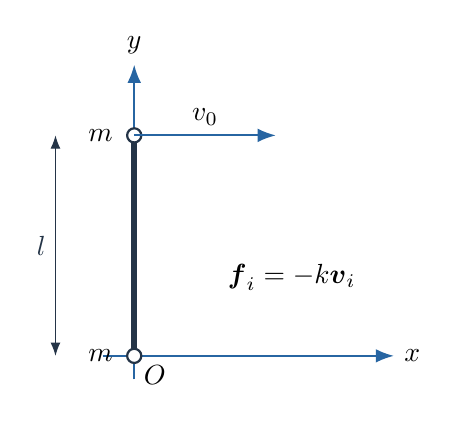
\begin{tikzpicture}
\draw[vec](-.4,0)--(3.3,0)node[right]{$x$};\draw[vec](0,-.3)--(0,3.7)node[above]{$y$};
\draw[body,line width=2pt](0,0)--(0,2.8);
\foreach \y in {0,2.8}{\draw[body,fill=white](0,\y)circle(.09);\node[left]at(-.15,\y){$m$};}
\draw[vec](0,2.8)--(1.8,2.8)node[midway,above]{$v_0$};
\draw[dim](-1,0)--(-1,2.8)node[midway,left]{$l$};
\node[below right]at(0,0){$O$};\node at(2,1){$\boldsymbol f_i=-k\boldsymbol v_i$};
\end{tikzpicture}
\begin{tikzpicture}
\draw[body](0,0)--(0,3);
\fill[ink](0,1.5)circle(.045)node[left]{$C$};
\foreach \y in {0,3}{\draw[body,fill=white](0,\y)circle(.07);}
\draw[vec](0,3.35)--(1.8,3.35)node[midway,above]{$v_0$};
\draw[vec](0,1.5)--(.9,1.5)node[right]{$V_{C0}=v_0/2$};
\draw[green,thick,-{Latex}](0,2.85)--(.9,2.85)node[right]{$v_0/2$};
\draw[green,thick,-{Latex}](0,.15)--(-.9,.15)node[left]{$v_0/2$};
\node[below]at(0,-.25){下端合速度为零};
\node[right]at(2.1,2.9){上端相对转动};
\draw[blue,-{Latex}](-.8,1.5)arc(180:-20:.8);
\node at(2.3,.8){$\Omega_0=-v_0/l$};
\end{tikzpicture}
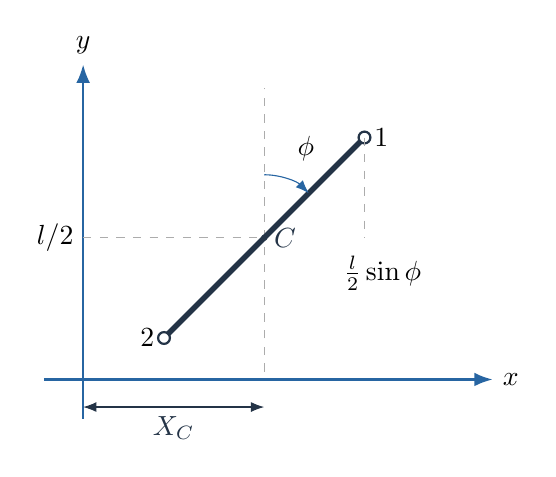
\begin{tikzpicture}
\draw[vec](-.5,0)--(5.2,0)node[right]{$x$};\draw[vec](0,-.5)--(0,4)node[above]{$y$};
\coordinate(C)at(2.3,1.8);\coordinate(U)at(3.573,3.073);\coordinate(D)at(1.027,.527);
\draw[guide](2.3,.1)--(2.3,3.7); \draw[guide](0,1.8)--(C);
\draw[body,line width=2pt](D)--(U);
\foreach \p in {U,D}{\draw[body,fill=white](\p)circle(.075);}
\fill[ink](C)circle(.04)node[right]{$C$};
\node[right]at(U){$1$};\node[left]at(D){$2$};
\draw[blue,-{Latex}]($(C)+(0,.8)$)arc(90:45:.8);
\node[above right]at(2.6,2.65){$\phi$};
\draw[dim](0,-.35)--(2.3,-.35)node[midway,below]{$X_C$};
\draw[guide](U)--(3.573,1.8);
\node at(3.8,1.35){$\frac l2\sin\phi$};
\node[left]at(0,1.8){$l/2$};
\end{tikzpicture}
\begin{tikzpicture}
\draw[vec](-.2,0)--(7.7,0)node[right]{$x_1/l$};\draw[vec](0,-.3)--(0,2.6)node[above]{$y_1/l$};
\draw[blue,thick,domain=0:285,samples=180,variable=\a]plot({\a*pi/180+sin(\a)},{1+cos(\a)});
\fill[blue](0,2)circle(.04)node[above right]{初态};
\fill[white,draw=red](pi,0)circle(.05)node[below,text=ink]{$\pi/2$};
\node[red]at(5,-.8){$\phi=\pi$：瞬时零速};
\node[left]at(0,2){$1$};
\end{tikzpicture}
\end{document}
